\documentclass{article}

\usepackage{fullpage}
\usepackage{siunitx}
\usepackage{graphicx}
\usepackage{hyperref}
\hypersetup{colorlinks=true, linkcolor=blue}
\usepackage{wrapfig}

\setlength{\parindent}{0pt}
\setlength{\parskip}{2ex plus 1ex minus 1ex}


\begin{document}

\appendix


\section{Copper}

The sample was the canonical copper foil of Newville, et al. fame.
The fitting model is very simple.  There is an S$_0^2$ parameter
(\texttt{amp}), an energy shift for all paths (\texttt{enot}), and a
volumetric lattice expansion coefficient (\texttt{alpha}).  The
$\sigma^2$ values for all paths were computed using the correlated
Debye model and a temperature of 10\,K, except for the first shell,
which has its own $\sigma^2$ variable (\texttt{ss1}).

The fit included 4 coordination shells, which includes several
collinear multiple scattering paths of the same distance as the fourth
shell single scattering path.

\texttt{amp} and \texttt{alpha} are unitless.  \texttt{enot} is eV,
\texttt{ss1} is \AA$^2$, and \texttt{thetad} is K.

\small
\input{Copper/Copper}

\newpage

\begin{minipage}{0.49\linewidth}
  \large Fit to Copper using \textsc{feff}6\\[3ex]
  \includegraphics[width=0.9\linewidth]{{Copper/fit_feff6}.png}
\end{minipage}
\begin{minipage}{0.49\linewidth}
  \large Fit to Copper using \textsc{feff}8.5, no SCF\\[3ex]
  \includegraphics[width=0.9\linewidth]{{Copper/fit_noSCF}.png}
\end{minipage}

\bigskip

\begin{minipage}{0.49\linewidth}
  \large Fit to Copper using \textsc{feff}8.5, SCF, R=3\,\AA\\[3ex]
  \includegraphics[width=0.9\linewidth]{{Copper/fit_withSCF_3}.png}
\end{minipage}
\begin{minipage}{0.49\linewidth}
  \large Fit to Copper using \textsc{feff}8.5, SCF, R=4\,\AA\\[3ex]
  \includegraphics[width=0.9\linewidth]{{Copper/fit_withSCF_4}.png}
\end{minipage}

\bigskip

\begin{minipage}{0.49\linewidth}
  \large Fit to Copper using \textsc{feff}8.5, SCF, R=5\,\AA\\[3ex]
  \includegraphics[width=0.9\linewidth]{{Copper/fit_withSCF_5}.png}
\end{minipage}
\begin{minipage}{0.49\linewidth}
  \large Fit to Copper using \textsc{feff}8.5, SCF, R=5\,\AA\\[3ex]
  \includegraphics[width=0.9\linewidth]{{Copper/fit_withSCF_5.5}.png}
\end{minipage}

\bigskip

\begin{minipage}{0.49\linewidth}
  \large Fit to Copper using \textsc{feff}8.5, SCF, R=6\,\AA\\[3ex]
  \includegraphics[width=0.9\linewidth]{{Copper/fit_withSCF_6}.png}
\end{minipage}

%%%%%%%%%%%%%%%%%%%%%%%%%%%%%%%%%%%%%%%%%%%%%%%%%%%%%%%%%%%%%%%%%%%%%%
%%%%%%%%%%%%%%%%%%%%%%%%%%%%%%%%%%%%%%%%%%%%%%%%%%%%%%%%%%%%%%%%%%%%%%
%%%%%%%%%%%%%%%%%%%%%%%%%%%%%%%%%%%%%%%%%%%%%%%%%%%%%%%%%%%%%%%%%%%%%%

\newpage

\section{NiO}

\normalsize

The sample was NiO powder prepared by my colleague Neil Hyatt
(University of Sheffield) and checked by him for phase purity.  The
powder was spread onto kapton tape and folded over to make a edge step
of 0.78.  The simple fiting model to this rocksalt structure included
a S$_0^2$ parameter (\texttt{amp}), an energy shift (\texttt{enot}),
and a volumetric lattice expansion coefficient (\texttt{alpha}).

The fit included 4 coordination shells, 2 with O and 2 with Ni.  There
are several collinear multiple scattering paths at the same distance
as the fourth shell Ni scatterer.  Each shell has its own $\sigma^2$
parameter (\texttt{sso}, \texttt{ssni}, \texttt{sso2}, and
\texttt{ssni2}, respectively.).

\texttt{amp} and \texttt{alpha} are unitless.  \texttt{enot} is eV.
\texttt{sso}, \texttt{ssni}, \texttt{sso2}, and \texttt{ssni2} are
\AA$^2$.

\small
\input{NiO/NiO}

\newpage

\begin{minipage}{0.49\linewidth}
  \large Fit to NiO using \textsc{feff}6\\[3ex]
  \includegraphics[width=0.9\linewidth]{{NiO/fit_feff6}.png}
\end{minipage}
\begin{minipage}{0.49\linewidth}
  \large Fit to NiO using \textsc{feff}8.5, no SCF\\[3ex]
  \includegraphics[width=0.9\linewidth]{{NiO/fit_noSCF}.png}
\end{minipage}

\bigskip

\begin{minipage}{0.49\linewidth}
  \large Fit to NiO using \textsc{feff}8.5, SCF, R=2.5\,\AA\\[3ex]
  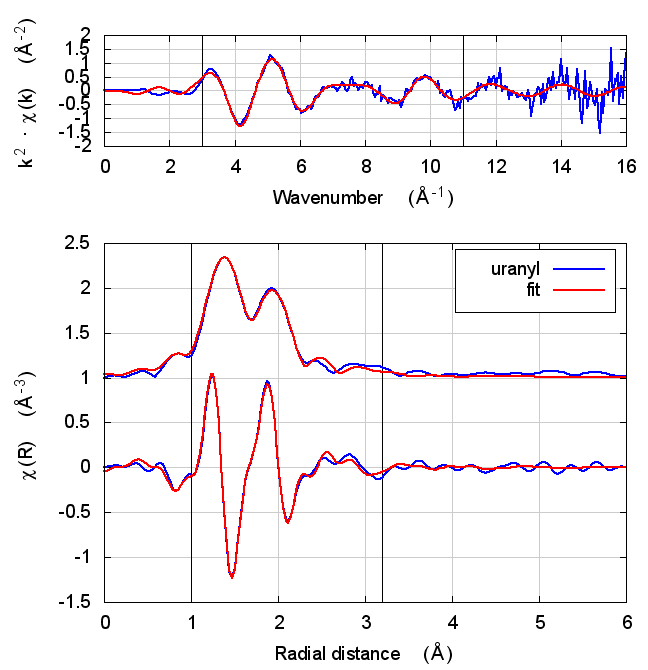
\includegraphics[width=0.9\linewidth]{{NiO/fit_withSCF_2.5}.png}
\end{minipage}
\begin{minipage}{0.49\linewidth}
  \large Fit to NiO using \textsc{feff}8.5, SCF, R=3\,\AA\\[3ex]
  \includegraphics[width=0.9\linewidth]{{NiO/fit_withSCF_3}.png}
\end{minipage}

\bigskip

\begin{minipage}{0.49\linewidth}
  \large Fit to NiO using \textsc{feff}8.5, SCF, R=3.7\,\AA\\[3ex]
  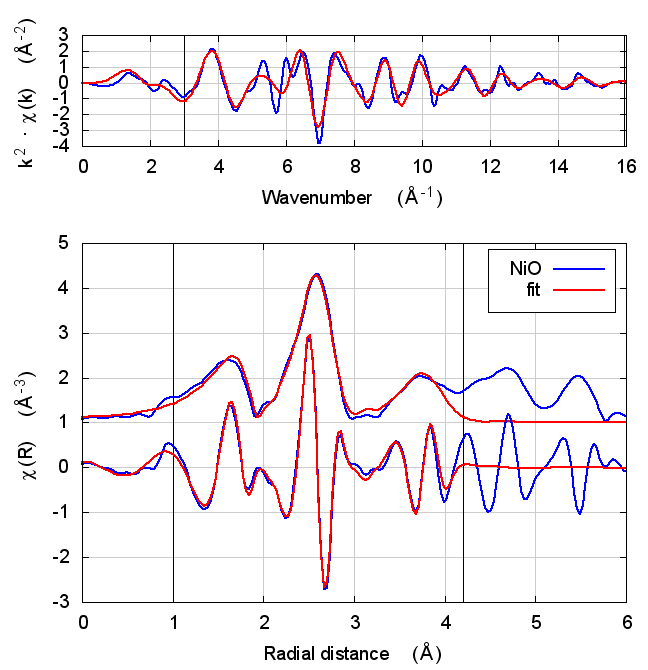
\includegraphics[width=0.9\linewidth]{{NiO/fit_withSCF_3.7}.png}
\end{minipage}
\begin{minipage}{0.49\linewidth}
  \large Fit to NiO using \textsc{feff}8.5, SCF, R=4.2\,\AA\\[3ex]
  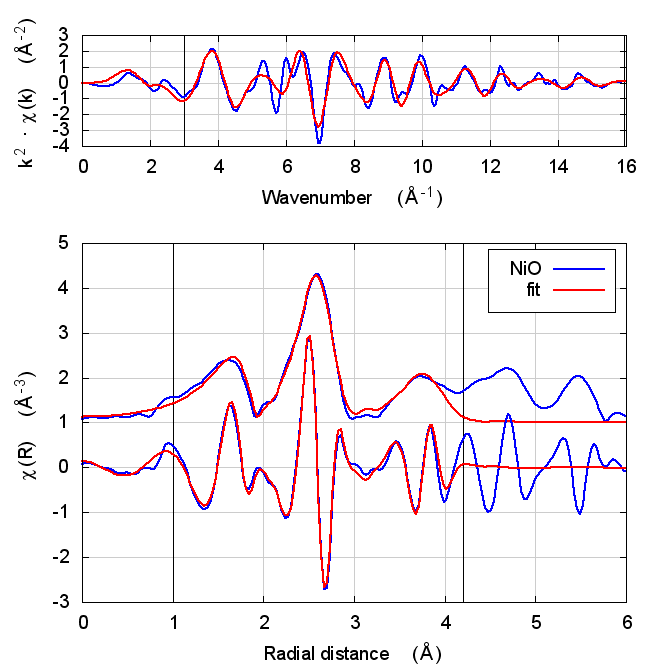
\includegraphics[width=0.9\linewidth]{{NiO/fit_withSCF_4.2}.png}
\end{minipage}

\bigskip

\begin{minipage}{0.49\linewidth}
  \large Fit to NiO using \textsc{feff}8.5, SCF, R=4.7\,\AA\\[3ex]
  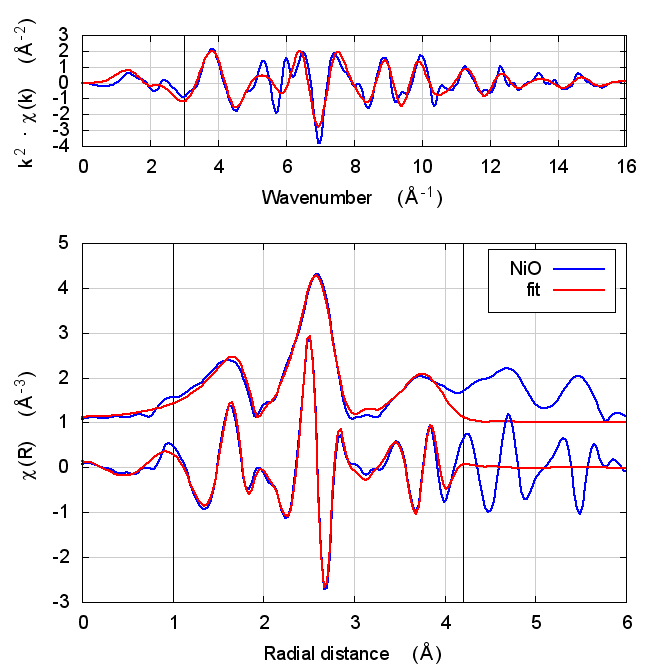
\includegraphics[width=0.9\linewidth]{{NiO/fit_withSCF_4.7}.png}
\end{minipage}


%%%%%%%%%%%%%%%%%%%%%%%%%%%%%%%%%%%%%%%%%%%%%%%%%%%%%%%%%%%%%%%%%%%%%%
%%%%%%%%%%%%%%%%%%%%%%%%%%%%%%%%%%%%%%%%%%%%%%%%%%%%%%%%%%%%%%%%%%%%%%
%%%%%%%%%%%%%%%%%%%%%%%%%%%%%%%%%%%%%%%%%%%%%%%%%%%%%%%%%%%%%%%%%%%%%%

\newpage

\section{FeS$_2$}
\normalsize

This is one of my standard teaching examples.  It's good for teaching
as it is fairly simple -- it's cubic -- but it has a bit of structure
and a two kinds of scatterers.  The data are taken from Matt's online
collection of references.

The model includes a S$_0^2$ parameter (\texttt{amp}), an energy shift
(\texttt{enot}), and a volumetric lattice expansion coefficient
(\texttt{alpha}).  The first and second shell S scatterers each get a
$\sigma^2$ parameter (\texttt{ss} and \texttt{ss2}).  The third shell
of S atoms only contains 2 scatterers.  In practice, floating its
$\sigma^2$ parameter independently does not yeild a statistical
improvment to the fit, so the \texttt{ss2} parameter is used for the
third shell $\sigma^2$.  Finally a $\sigma^2$ parameter is floated for
the Fe shell.

The fitting model includes a variety of multiple scattering paths,
including a triangle between the first shell S and the fourth shell
Fe, and four paths that bounce around among first shell S atoms.

\texttt{amp} and \texttt{alpha} are unitless.  \texttt{enot} is eV.
\texttt{ss}, \texttt{ss2}, and \texttt{ssfe} are \AA$^2$.

\small
\input{FeS2/FeS2}

\newpage


\begin{minipage}{0.49\linewidth}
  \large Fit to FeS$_2$ using \textsc{feff}6\\[3ex]
  \includegraphics[width=0.9\linewidth]{{FeS2/fit_feff6}.png}
\end{minipage}
\begin{minipage}{0.49\linewidth}
  \large Fit to FeS$_2$ using \textsc{feff}8.5, no SCF\\[3ex]
  \includegraphics[width=0.9\linewidth]{{FeS2/fit_noSCF}.png}
\end{minipage}

\bigskip

\begin{minipage}{0.49\linewidth}
  \large Fit to FeS$_2$ using \textsc{feff}8.5, SCF, R=3\,\AA\\[3ex]
  \includegraphics[width=0.9\linewidth]{{FeS2/fit_withSCF_3}.png}
\end{minipage}
\begin{minipage}{0.49\linewidth}
  \large Fit to FeS$_2$ using \textsc{feff}8.5, SCF, R=3.6\,\AA\\[3ex]
  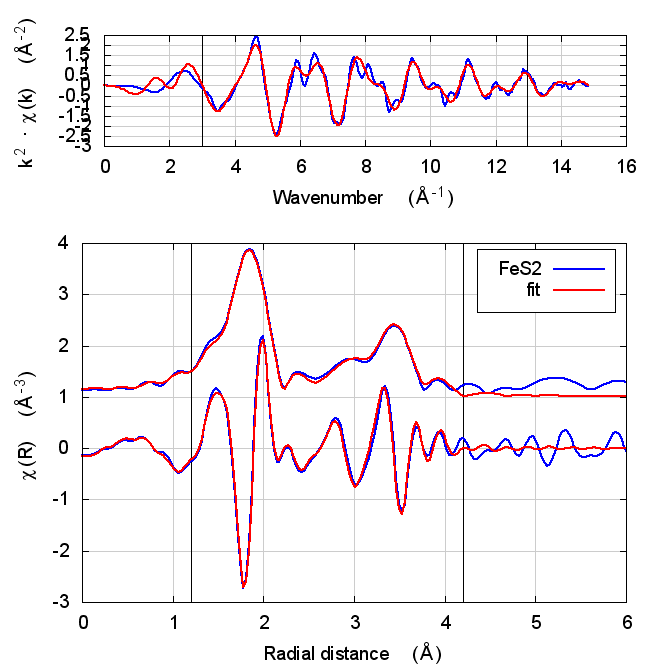
\includegraphics[width=0.9\linewidth]{{FeS2/fit_withSCF_3.6}.png}
\end{minipage}

\bigskip

\begin{minipage}{0.49\linewidth}
  \large Fit to FeS$_2$ using \textsc{feff}8.5, SCF, R=4\,\AA\\[3ex]
  \includegraphics[width=0.9\linewidth]{{FeS2/fit_withSCF_4}.png}
\end{minipage}
\begin{minipage}{0.49\linewidth}
  \large Fit to FeS$_2$ using \textsc{feff}8.5, SCF, R=5.3\,\AA\\[3ex]
  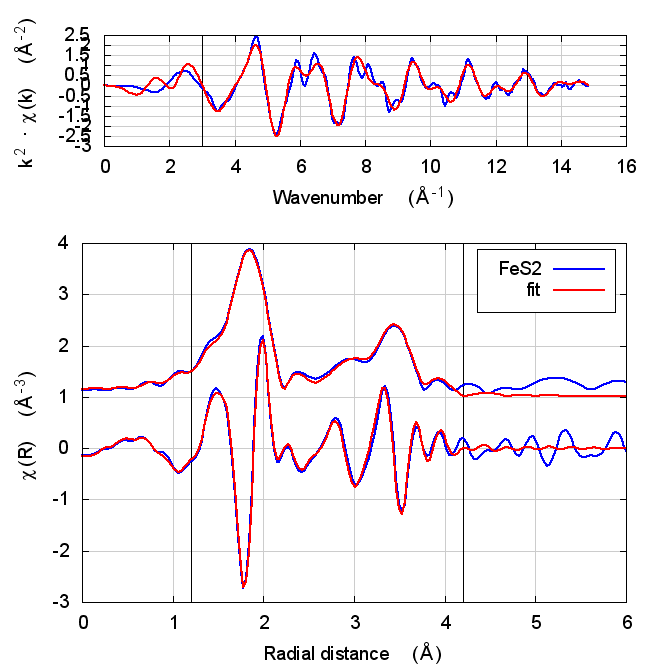
\includegraphics[width=0.9\linewidth]{{FeS2/fit_withSCF_5.3}.png}
\end{minipage}

\bigskip

\begin{minipage}{0.49\linewidth}
  \large Fit to FeS$_2$ using \textsc{feff}8.5, SCF, R=5.5\,\AA\\[3ex]
  \includegraphics[width=0.9\linewidth]{{FeS2/fit_withSCF_5.5}.png}
\end{minipage}


%%%%%%%%%%%%%%%%%%%%%%%%%%%%%%%%%%%%%%%%%%%%%%%%%%%%%%%%%%%%%%%%%%%%%%
%%%%%%%%%%%%%%%%%%%%%%%%%%%%%%%%%%%%%%%%%%%%%%%%%%%%%%%%%%%%%%%%%%%%%%
%%%%%%%%%%%%%%%%%%%%%%%%%%%%%%%%%%%%%%%%%%%%%%%%%%%%%%%%%%%%%%%%%%%%%%

\newpage

\section{UO$_2$}
\normalsize

\begin{wrapfigure}{r}{0.25\textwidth}
  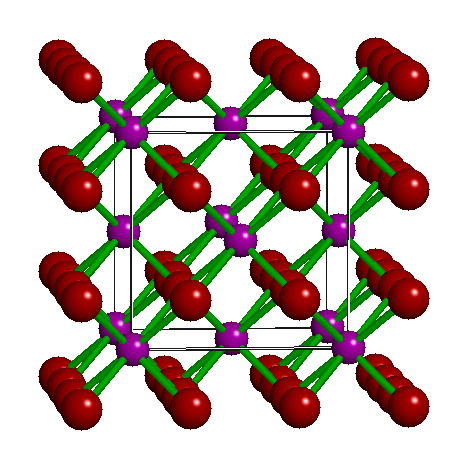
\includegraphics[width=\linewidth]{UO2/UO2.png}
  \caption{Uraninite}
\end{wrapfigure}
The data are the UO$_2$ shown in Shelly's paper on \textit{Reduction
  of Uranium(VI) by Mixed Iron(II)/Iron(III) Hydroxide (Green Rust): 
  Formation of UO$_2$ Nanoparticles}:
\href{http://dx.doi.org/10.1021/es0208409}{\texttt{http://dx.doi.org/10.1021/es0208409}}

The fitting model follows rather closely to what is described in that
paper, particularly the content of Table 2, although I allow S$_0^2$
to float (\texttt{amp}).  Along with an energy shift (\texttt{enot}),
a $\Delta R$ and $\sigma^2$ for the first shell O (\texttt{dro} and
\texttt{sso}), a $\Delta R$ and $\sigma^2$ for the second shell U
(\texttt{dru} and \texttt{ssu}), and a $\Delta R$ and $\sigma^2$ for
the third shell O (\texttt{dro2} and \texttt{sso2}), there is a
parameter for the number of U scatterers (\texttt{nu}).

The model includes the same 6 paths given in Table 2 of Shelly's
paper.

\texttt{amp} is unitless.  \texttt{enot} is eV.
\texttt{dro}, \texttt{dru}, and \texttt{dro2} are \AA.
\texttt{sso}, \texttt{ssu}, and \texttt{sso2} are \AA$^2$.


\scriptsize
\input{UO2/UO2}

\newpage

\begin{minipage}{0.49\linewidth}
  \large Fit to UO$_2$ using \textsc{feff}6\\[3ex]
  \includegraphics[width=0.9\linewidth]{{UO2/fit_feff6}.png}
\end{minipage}
\begin{minipage}{0.49\linewidth}
  \large Fit to UO$_2$ using \textsc{feff}8.5, no SCF\\[3ex]
  \includegraphics[width=0.9\linewidth]{{UO2/fit_noSCF}.png}
\end{minipage}

\bigskip

\begin{minipage}{0.49\linewidth}
  \large Fit to UO$_2$ using \textsc{feff}8.5, SCF, R=3\,\AA\\[3ex]
  \includegraphics[width=0.9\linewidth]{{UO2/fit_withSCF_3}.png}
\end{minipage}
\begin{minipage}{0.49\linewidth}
  \large Fit to UOS$_2$ using \textsc{feff}8.5, SCF, R=4\,\AA\\[3ex]
  \includegraphics[width=0.9\linewidth]{{UO2/fit_withSCF_4}.png}
\end{minipage}

\bigskip

\begin{minipage}{0.49\linewidth}
  \large Fit to UO$_2$ using \textsc{feff}8.5, SCF, R=5\,\AA\\[3ex]
  \includegraphics[width=0.9\linewidth]{{UO2/fit_withSCF_5}.png}
\end{minipage}
\begin{minipage}{0.49\linewidth}
  \large Fit to UOS$_2$ using \textsc{feff}8.5, SCF, R=5.5\,\AA\\[3ex]
  \includegraphics[width=0.9\linewidth]{{UO2/fit_withSCF_5.5}.png}
\end{minipage}

\bigskip

\begin{minipage}{0.49\linewidth}
  \large Fit to UO$_2$ using \textsc{feff}8.5, SCF, R=6\,\AA\\[3ex]
  \includegraphics[width=0.9\linewidth]{{UO2/fit_withSCF_6}.png}
\end{minipage}


%%%%%%%%%%%%%%%%%%%%%%%%%%%%%%%%%%%%%%%%%%%%%%%%%%%%%%%%%%%%%%%%%%%%%%
%%%%%%%%%%%%%%%%%%%%%%%%%%%%%%%%%%%%%%%%%%%%%%%%%%%%%%%%%%%%%%%%%%%%%%
%%%%%%%%%%%%%%%%%%%%%%%%%%%%%%%%%%%%%%%%%%%%%%%%%%%%%%%%%%%%%%%%%%%%%%

\newpage

\section{BaZrO$_3$}
\normalsize


\begin{wrapfigure}{r}{0.25\textwidth}
  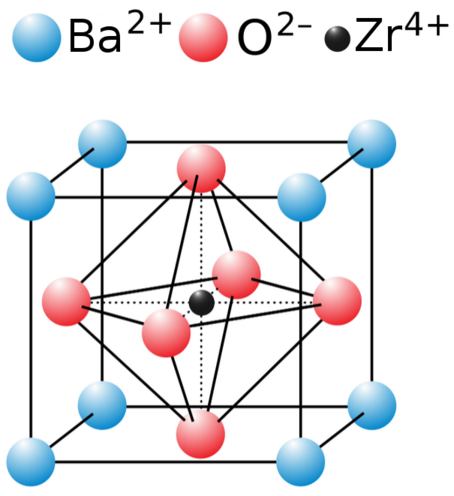
\includegraphics[width=\linewidth]{BaZrO3/perovskite.png}
  \caption{The perovskite structure.}
\end{wrapfigure}
In this paper on the Zr edge of BaZrO$_3$
\href{http://dx.doi.org/10.1016/0921-4526(94)00654-E}
{\texttt{http://dx.doi.org/10.1016/0921-4526(94)00654-E}}, Haskel et
al. (and what a sordid ``et al.'' \textit{that} was) proposed that
shortcomings of \textsc{feff}'s potential model could be accommodated
by floating an energy shift parameter for each scatterer species.  The
concept is that doing so approximates the effect if errors in the
scattering phase shifts.

The data are the same as in that paper, although the fitting model is
slightly different.  Rather than floating $\Delta R$ parameters for
each shell, I used a volumetric expansion coefficient
(\texttt{alpha}).  Along with S$_0^2$ (\texttt{amp}), there are energy
shofts for each scatterer (\texttt{enot}, \texttt{ezr}, and
\texttt{eba}) and $\sigma^2$ parameters for each scatterer
(\texttt{sso}, \texttt{sszr}, and \texttt{ssba}.  The fourth shell O
is included in the fit.  It gets a $\sigma^2$ (\texttt{sso2})but uses
the energy shift for the O scatterer.

BaZrO$_3$ is a true perovskite.  Zr sites in the octahedral B site.  A
variety of collinear multiple scattering paths at the distance of the
third shell Zr scatterer are included in the fit.  The energy shifts
are parameterized as described in the paper.

\texttt{amp} and \texttt{alpha} are unitless.  \texttt{enot},
\texttt{ezr}, and \texttt{eba} are eV.  \texttt{sso}, \texttt{sszr},
\texttt{ssba}, and \texttt{sso2} are \AA$^2$.

\scriptsize
\input{BaZrO3/BaZrO3}

\newpage


\begin{minipage}{0.49\linewidth}
  \large Fit to BaZrO$_3$ using \textsc{feff}6\\[3ex]
  \includegraphics[width=0.9\linewidth]{{BaZrO3/fit_feff6}.png}
\end{minipage}
\begin{minipage}{0.49\linewidth}
  \large Fit to BaZrO$_3$ using \textsc{feff}8.5, no SCF\\[3ex]
  \includegraphics[width=0.9\linewidth]{{BaZrO3/fit_noSCF}.png}
\end{minipage}

\bigskip

\begin{minipage}{0.49\linewidth}
  \large Fit to BaZrO$_3$ using \textsc{feff}8.5, SCF, R=3\,\AA\\[3ex]
  \includegraphics[width=0.9\linewidth]{{BaZrO3/fit_withSCF_3}.png}
\end{minipage}
\begin{minipage}{0.49\linewidth}
  \large Fit to BaZrO$_3$ using \textsc{feff}8.5, SCF, R=4\,\AA\\[3ex]
  \includegraphics[width=0.9\linewidth]{{BaZrO3/fit_withSCF_4}.png}
\end{minipage}

\bigskip

\begin{minipage}{0.49\linewidth}
  \large Fit to BaZrO$_3$ using \textsc{feff}8.5, SCF, R=5\,\AA\\[3ex]
  \includegraphics[width=0.9\linewidth]{{BaZrO3/fit_withSCF_5}.png}
\end{minipage}
\begin{minipage}{0.49\linewidth}
  \large Fit to BaZrO$_3$ using \textsc{feff}8.5, SCF, R=5.5\,\AA\\[3ex]
  \includegraphics[width=0.9\linewidth]{{BaZrO3/fit_withSCF_5.5}.png}
\end{minipage}

\bigskip

\begin{minipage}{0.49\linewidth}
  \large Fit to BaZrO$_3$ using \textsc{feff}8.5, SCF, R=6\,\AA\\[3ex]
  \includegraphics[width=0.9\linewidth]{{BaZrO3/fit_withSCF_6}.png}
\end{minipage}

%%%%%%%%%%%%%%%%%%%%%%%%%%%%%%%%%%%%%%%%%%%%%%%%%%%%%%%%%%%%%%%%%%%%%%
%%%%%%%%%%%%%%%%%%%%%%%%%%%%%%%%%%%%%%%%%%%%%%%%%%%%%%%%%%%%%%%%%%%%%%
%%%%%%%%%%%%%%%%%%%%%%%%%%%%%%%%%%%%%%%%%%%%%%%%%%%%%%%%%%%%%%%%%%%%%%

% \newpage

% \section{methyltin}
% \normalsize

% \small
% \input{methyltin/methyltin}

% \newpage

%%%%%%%%%%%%%%%%%%%%%%%%%%%%%%%%%%%%%%%%%%%%%%%%%%%%%%%%%%%%%%%%%%%%%%
%%%%%%%%%%%%%%%%%%%%%%%%%%%%%%%%%%%%%%%%%%%%%%%%%%%%%%%%%%%%%%%%%%%%%%
%%%%%%%%%%%%%%%%%%%%%%%%%%%%%%%%%%%%%%%%%%%%%%%%%%%%%%%%%%%%%%%%%%%%%%

\newpage

\section{bromoadamantane}
\normalsize


\begin{wrapfigure}{r}{0.25\textwidth}
  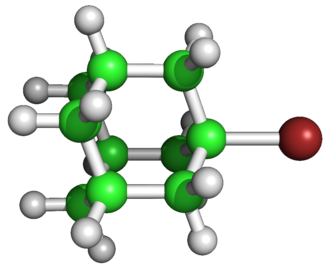
\includegraphics[width=\linewidth]{bromoadamantane/bromoadamantane.png}
  \caption{~\hfill\break 1-bromoadamantane}
\end{wrapfigure}

The data are 1-bromoadamantane.  Adamanatane is a cycloalkane, meaning
that it is a hydrocarbon with rings of carbon atoms.  It is also a
diamondoid, meaning that it is a strong, stiff, 3D network of covalent
bonds.  1-bromoadamantane has one hydrogen atom replaced by a bromine
atom.

The material was supplied by my colleague Alessandra Leri of Manhattan
Marymount College in the form of a white powder.  This powder was
spread onto kapton tape which was folded to make a sample with an edge
step of about 1.7.

This is an interesting test case becasue it is a molecule (thus the
entire molecule can be included in the self-consistency calculation)
and because there is measureable scattering from the neighboring
hydrogen atoms.  While the $\sigma^2$ of the hydrogen scatterers is not
well-determined, the fit is statistically significantly worse when the
hydrogen scatterers are excluded.

The fit includes the nearest neighbor C, the next three C atoms, and
the neighboring 6 hydrogen atoms.  The DS triangle paths involving the
first and second neighbor C atoms are also included.  The fitting
model assumes that the adamanatane anion is very rigid compared to the
Br-C bond.  Thus, the formula explained in 
\href{http://dx.doi.org/10.1088/1742-6596/190/1/012026}%
{\texttt{http://dx.doi.org/10.1088/1742-6596/190/1/012026}} is used to
constrain the second neighbor C distance to the first neighbor C
$\Delta R$ parameter.


\small
\input{bromoadamantane/bromoadamantane}

\newpage

\begin{minipage}{0.49\linewidth}
  \large Fit to bromoadamantane using \textsc{feff}6\\[3ex]
  \includegraphics[width=0.9\linewidth]{{bromoadamantane/fit_feff6}.png}
\end{minipage}
\begin{minipage}{0.49\linewidth}
  \large Fit to bromoadamantane using \textsc{feff}8.5, no SCF\\[3ex]
  \includegraphics[width=0.9\linewidth]{{bromoadamantane/fit_noSCF}.png}
\end{minipage}

\bigskip

\begin{minipage}{0.49\linewidth}
  \large Fit to bromoadamantane using \textsc{feff}8.5, SCF, R=8\,\AA\\[3ex]
  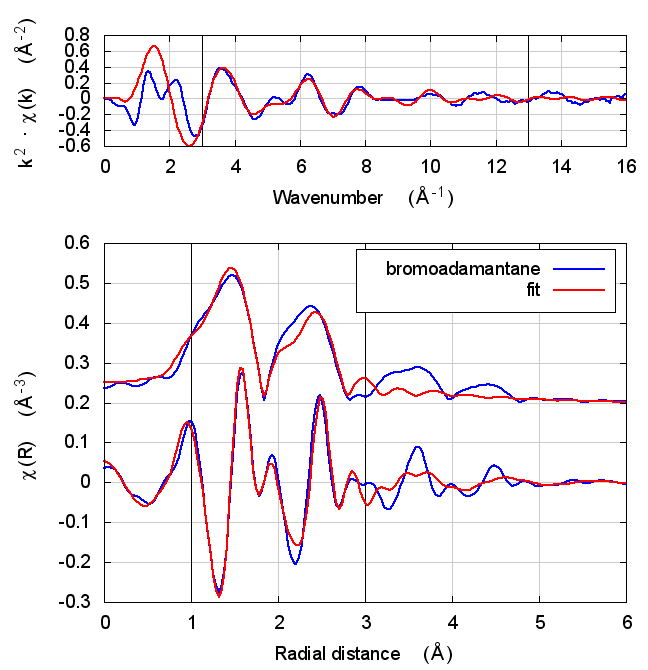
\includegraphics[width=0.9\linewidth]{{bromoadamantane/fit_withSCF_8}.png}
\end{minipage}


%%%%%%%%%%%%%%%%%%%%%%%%%%%%%%%%%%%%%%%%%%%%%%%%%%%%%%%%%%%%%%%%%%%%%%
%%%%%%%%%%%%%%%%%%%%%%%%%%%%%%%%%%%%%%%%%%%%%%%%%%%%%%%%%%%%%%%%%%%%%%
%%%%%%%%%%%%%%%%%%%%%%%%%%%%%%%%%%%%%%%%%%%%%%%%%%%%%%%%%%%%%%%%%%%%%%

\newpage

\section{uranyl}
\normalsize

\begin{wrapfigure}{r}{0.25\textwidth}
  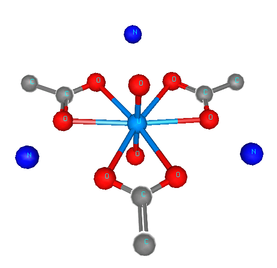
\includegraphics[width=\linewidth]{uranyl/uranyl.png}
  \caption{The uranyl motif from sodium uranyl triacetate.}
\end{wrapfigure}

The data are the uranyl hydrate shown in Shelly's paper on
\textit{X-ray absorption fine structure determination of pH-dependent
  U-bacterial cell wall interactions},
\href{http://dx.doi.org/10.1016/S0016-7037(02)00947-X}
{\texttt{http://dx.doi.org/10.1016/S0016-7037(02)00947-X}}

This is an interesting test case because it involves very short
($\sim1.78$\,\AA) uranium-oxygen bonds.  The \texttt{AFOLP} card was
used to run \textsc{feff}6.  The \texttt{FOLP} card with a value of
0.9 for each potential was used to get \textsc{feff}8.5 to run to
completion.

Following the lead of that paper, \textsc{feff} was run on the crystal
sodium uranyl triacetate.  The relevant bit of the structure is shown
in the figure.  For the fitting model, scattering paths related to the
axial and equatorial O atoms (red balls) are used in the fit.  Other
paths are unused.  The parameterization given in Tables 2 and 5 is
used in this fit.

There is an S$_0^2$ (\texttt{amp}) and an energy shift
(\texttt{enot}).  The axial and equatorial oxyegn atoms each get a
$\Delta R$ (\texttt{deloax} and \texttt{deloeq}) and a $\sigma^2$
(\texttt{sigoax} and \texttt{sigoeq}).

\texttt{amp} is unitless.  \texttt{enot} is eV.
\texttt{deloax} and \texttt{deloeq} are \AA.
\texttt{sigoax} and \texttt{sigoeq} are \AA$^2$.

\small
\input{uranyl/uranyl}

\newpage

\begin{minipage}{0.49\linewidth}
  \large Fit to uranyl using \textsc{feff}6\\[3ex]
  \includegraphics[width=0.9\linewidth]{{uranyl/fit_feff6}.png}
\end{minipage}
\begin{minipage}{0.49\linewidth}
  \large Fit to uranyl using \textsc{feff}8.5, no SCF\\[3ex]
  \includegraphics[width=0.9\linewidth]{{uranyl/fit_noSCF}.png}
\end{minipage}

\bigskip

\begin{minipage}{0.49\linewidth}
  \large Fit to uranyl using \textsc{feff}8.5, SCF, R=2.5\,\AA\\[3ex]
  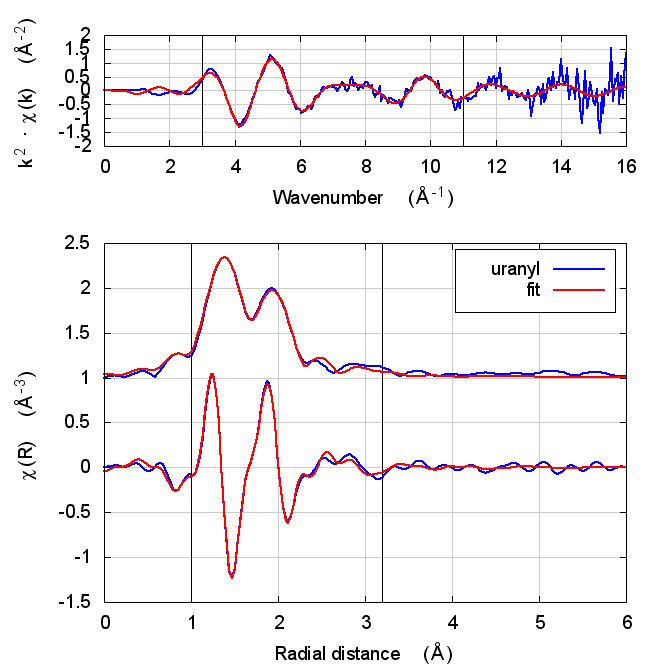
\includegraphics[width=0.9\linewidth]{{uranyl/fit_withSCF_2.9}.png}
\end{minipage}
\begin{minipage}{0.49\linewidth}
  \large Fit to uranyl using \textsc{feff}8.5, SCF, R=4\,\AA\\[3ex]
  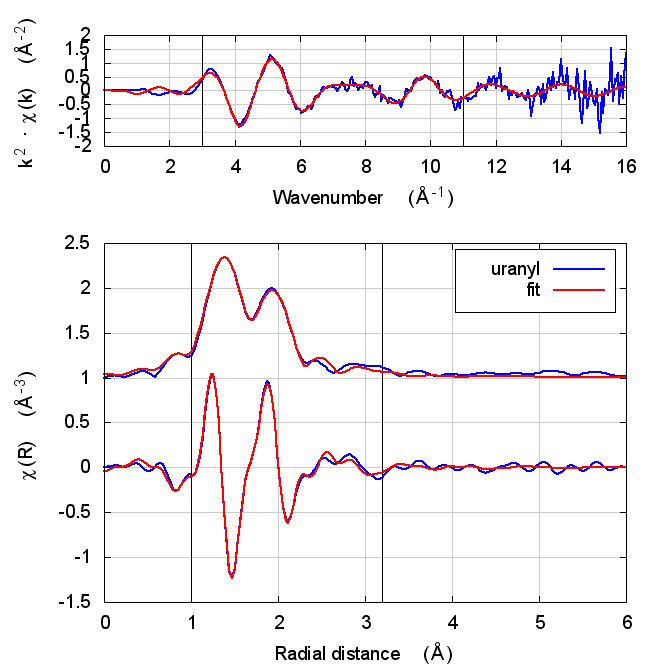
\includegraphics[width=0.9\linewidth]{{uranyl/fit_withSCF_2.9}.png}
\end{minipage}

\bigskip

\begin{minipage}{0.49\linewidth}
  \large Fit to uranyl using \textsc{feff}8.5, SCF, R=4.0\,\AA\\[3ex]
  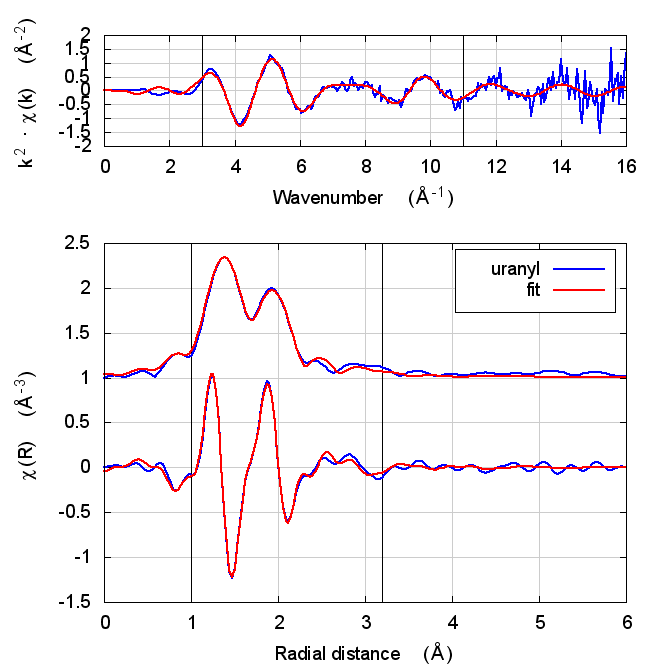
\includegraphics[width=0.9\linewidth]{{uranyl/fit_withSCF_4.0}.png}
\end{minipage}
\begin{minipage}{0.49\linewidth}
  \large Fit to uranyl using \textsc{feff}8.5, SCF, R=5.2\,\AA\\[3ex]
  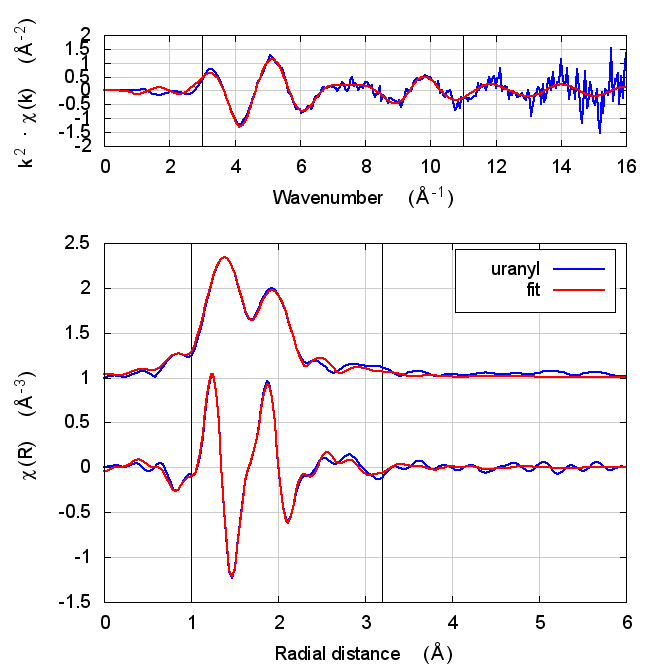
\includegraphics[width=0.9\linewidth]{{uranyl/fit_withSCF_5.2}.png}
\end{minipage}

\bigskip

\begin{minipage}{0.49\linewidth}
  \large Fit to uranyl using \textsc{feff}8.5, SCF, R=6.8\,\AA\\[3ex]
  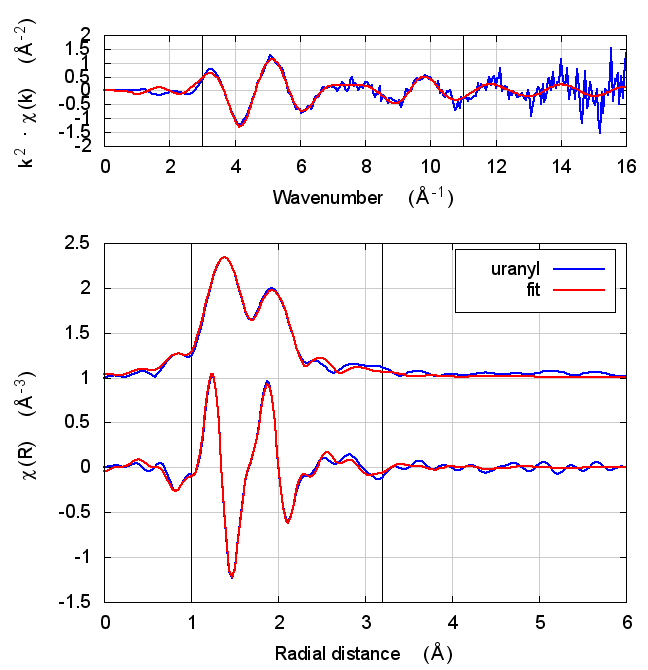
\includegraphics[width=0.9\linewidth]{{uranyl/fit_withSCF_6.8}.png}
\end{minipage}

\end{document}



%%% Local Variables:
%%% mode: latex
%%% TeX-master: t
%%% TeX-parse-self: t
%%% TeX-auto-save: t
%%% TeX-auto-untabify: t
%%% TeX-PDF-mode: t
%%% End:
